\begin{enumerate}[label=\thesubsection.\arabic*, ref=\thesubsection.\theenumi]

\item If $x = \alpha$ is a root of $p(x) = ax^2 + bx + c = 0$, then $p(\alpha) = 0$, i.e.,
\begin{align}
	\myvec{\alpha^2 & \alpha & 1}\myvec{a \\ b \\ c} = a\alpha^2 + b\alpha + c = 0
	\label{eq:EE26BTECH11225-root}
\end{align}

\item If $\alpha$ and $\beta$ are distinct zeroes of $p(x)$, then $\brak{x - \alpha}\brak{x - \beta}$ is a factor of $p(x)$.
\begin{align}
	p\brak{x} = \brak{x - \alpha}\brak{x - \beta}q\brak{x}
	\label{eq:EE26BTECH11225-factor}
\end{align}
\solution
Dividing $p\brak{x}$ by $\brak{x - \alpha}$,
\begin{align}
	p\brak{x} = \brak{x - \alpha}s\brak{x} + p\brak{\alpha}
	= \brak{x - \alpha}s\brak{x}
\end{align}
since $p\brak{\alpha} = 0$. Substituting $x = \beta$,
\begin{align}
	p\brak{\beta} = \brak{\beta - \alpha}s\brak{\beta} = 0
	\implies s\brak{\beta} = 0
\end{align}
as $\beta \neq \alpha$. Repeating the division for $s\brak{x}$ with the zero $\beta$ gives
$s\brak{x} = \brak{x - \beta}q\brak{x}$, yielding \eqref{eq:EE26BTECH11225-factor}.

\item Roots of a quadratic equation $ax^2 + bx + c = 0$ $\brak{a \neq 0}$ and nature of roots, with discriminant $D = b^2 - 4ac$:
\begin{align}
	x &= \frac{-b \pm \sqrt{D}}{2a}
	\label{eq:EE26BTECH11225-quadratic}
	\\
	\begin{cases}
		D > 0 & \implies \text{two distinct real roots} \\
		D = 0 & \implies \text{two equal real roots} \\
		D < 0 & \implies \text{no real roots}
	\end{cases}
	\nonumber
\end{align}
\solution
Dividing by $a$ and completing the square,
\begin{align}
	x^2 + \frac{b}{a}x + \frac{c}{a} = 0
	\implies \brak{x + \frac{b}{2a}}^2 = \frac{b^2 - 4ac}{4a^2}
\end{align}
Taking the square root on both sides yields \eqref{eq:EE26BTECH11225-quadratic}. The roots are real only if $D \geq 0$. Further, for roots $\alpha, \beta$,
\begin{align}
	\alpha + \beta = -\frac{b}{a}, \quad \alpha\beta = \frac{c}{a}
\end{align}
which also follows from the fact that $\alpha, \beta$ are the eigenvalues of the companion matrix
\begin{align}
	\vec{C} = \myvec{0 & 1 \\ -\frac{c}{a} & -\frac{b}{a}},
	\quad
	\mydet{\vec{C} - \lambda\vec{I}} = \lambda^2 + \frac{b}{a}\lambda + \frac{c}{a}
\end{align}
with $\sum \lambda_i = \text{Tr}\brak{\vec{C}}$ and $\prod \lambda_i = \mydet{\vec{C}}$.

\item The $n^{\text{th}}$ term $a_n$ of an Arithmetic Progression (A.P.) with first term $a$ and common difference $d$:
\begin{align}
	a_n = a + \brak{n - 1}d
	\label{eq:EE26BTECH11225-ap-nth}
\end{align}
\solution
By definition $a_{k+1} - a_k = d$. Summing for $k = 1, 2, \ldots, n-1$ (telescoping),
\begin{align}
	\sum_{k=1}^{n-1}\brak{a_{k+1} - a_k} = a_n - a_1 = \brak{n - 1}d
\end{align}
and $a_1 = a$, yielding \eqref{eq:EE26BTECH11225-ap-nth}.

\item Sum of the first $n$ terms $S_n$ of an A.P.:
\begin{align}
	S_n = \frac{n}{2}\sbrak{2a + \brak{n - 1}d} = \frac{n}{2}\brak{a + l}
	\label{eq:EE26BTECH11225-ap-sum}
\end{align}
where $l = a_n$ is the last term.
\\
\solution
Writing the sum forwards and backwards,
\begin{align}
	S_n &= a_1 + a_2 + \cdots + a_n
	\\
	S_n &= a_n + a_{n-1} + \cdots + a_1
\end{align}
From \eqref{eq:EE26BTECH11225-ap-nth}, each pair satisfies
$a_k + a_{n+1-k} = 2a + \brak{n-1}d = a + l$. Adding the two equations,
\begin{align}
	2S_n = n\brak{a + l} = n\sbrak{2a + \brak{n - 1}d}
\end{align}
yielding \eqref{eq:EE26BTECH11225-ap-sum}.

\item Four consecutive terms in an A.P. with common difference $2d$:
\begin{align}
	\myvec{a - 3d \\ a - d \\ a + d \\ a + 3d}
	= a\vec{1} + d\myvec{-3 \\ -1 \\ 1 \\ 3}
	\label{eq:EE26BTECH11225-ap-four}
\end{align}
where $\vec{1}$ is the all-ones vector.
\\
\solution
The difference between any two consecutive entries is
\begin{align}
	\brak{a - d} - \brak{a - 3d} = \brak{a + d} - \brak{a - d} = \brak{a + 3d} - \brak{a + d} = 2d
\end{align}
and the mean of the four terms is $a$, which is why this choice simplifies the equations.

\item Distance between the points $\vec{P} = \myvec{x_1 \\ y_1}$ and $\vec{Q} = \myvec{x_2 \\ y_2}$:
\begin{align}
	d = \norm{\vec{Q} - \vec{P}}
	= \sqrt{\brak{\vec{Q} - \vec{P}}^{\top}\brak{\vec{Q} - \vec{P}}}
	= \sqrt{\brak{x_2 - x_1}^2 + \brak{y_2 - y_1}^2}
	\label{eq:EE26BTECH11225-distance}
\end{align}
\solution
The direction vector from $\vec{P}$ to $\vec{Q}$ is
\begin{align}
	\vec{Q} - \vec{P} = \myvec{x_2 - x_1 \\ y_2 - y_1}
\end{align}
and its length is the norm, obtained from the Pythagoras theorem, yielding \eqref{eq:EE26BTECH11225-distance}.

\item Section formula: the point $\vec{R}$ dividing the line joining $\vec{P}$ and $\vec{Q}$ internally in the ratio $k : 1$ is
\begin{align}
	\vec{R} = \frac{k\vec{Q} + \vec{P}}{k + 1}
	\iff
	\myvec{x \\ y} = \frac{1}{k + 1}\myvec{k x_2 + x_1 \\ k y_2 + y_1}
	\label{eq:EE26BTECH11225-section}
\end{align}
\solution
Since $\vec{R}$ lies on the line segment $PQ$ with $PR : RQ = k : 1$,
\begin{align}
	\vec{R} - \vec{P} &= k\brak{\vec{Q} - \vec{R}}
	\\
	\implies \brak{k + 1}\vec{R} &= k\vec{Q} + \vec{P}
\end{align}
yielding \eqref{eq:EE26BTECH11225-section}. For $k = 1$, $\vec{R}$ is the midpoint of $PQ$.

\item The area of a triangle with vertices $\vec{A} = \myvec{x_1 \\ y_1}$, $\vec{B} = \myvec{x_2 \\ y_2}$ and $\vec{C} = \myvec{x_3 \\ y_3}$ is
\begin{align}
	\text{Area}\brak{\Delta ABC}
	&= \frac{1}{2}\abs{\det\myvec{\vec{B} - \vec{A} & \vec{C} - \vec{A}}}
	\nonumber
	\\
	&= \frac{1}{2}\abs{x_1\brak{y_2 - y_3} + x_2\brak{y_3 - y_1} + x_3\brak{y_1 - y_2}}
	\label{eq:EE26BTECH11225-area-triangle}
\end{align}
The area of the quadrilateral $ABCD$, whose diagonal $AC$ lies inside it, is
\begin{align}
	\text{Area}\brak{ABCD} = \text{Area}\brak{\Delta ABC} + \text{Area}\brak{\Delta ADC}
	\label{eq:EE26BTECH11225-area-quad}
\end{align}
\solution
Let $\vec{a} = \vec{B} - \vec{A}$, $\vec{b} = \vec{C} - \vec{A}$ and let $\theta$ be the angle at $A$. Then
\begin{align}
	\text{Area}\brak{\Delta ABC} = \frac{1}{2}\norm{\vec{a}}\norm{\vec{b}}\sin\theta
\end{align}
Choosing $\vec{a} = \norm{\vec{a}}\myvec{\cos\phi \\ \sin\phi}$ and $\vec{b} = \norm{\vec{b}}\myvec{\cos\brak{\phi + \theta} \\ \sin\brak{\phi + \theta}}$,
\begin{align}
	\det\myvec{\vec{a} & \vec{b}}
	&= \norm{\vec{a}}\norm{\vec{b}}\sbrak{\cos\phi\sin\brak{\phi + \theta} - \sin\phi\cos\brak{\phi + \theta}}
	\\
	&= \norm{\vec{a}}\norm{\vec{b}}\sin\theta
\end{align}
Expanding the determinant,
\begin{align}
	\mydet{x_2 - x_1 & x_3 - x_1 \\ y_2 - y_1 & y_3 - y_1}
	= x_1\brak{y_2 - y_3} + x_2\brak{y_3 - y_1} + x_3\brak{y_1 - y_2}
\end{align}
yielding \eqref{eq:EE26BTECH11225-area-triangle}. The modulus accounts for the orientation of the vertices. The diagonal $AC$ splits $ABCD$ into $\Delta ABC$ and $\Delta ADC$, resulting in \eqref{eq:EE26BTECH11225-area-quad}.

\item Area Ratio Theorem for similar triangles $\Delta ABC \sim \Delta PQR$:
\begin{align}
	\frac{\text{ar}\brak{\Delta ABC}}{\text{ar}\brak{\Delta PQR}} = \brak{\frac{AB}{PQ}}^2
	\label{eq:EE26BTECH11225-area-ratio}
\end{align}
\solution
Similarity with scale factor $s = \frac{PQ}{AB}$ means there exist an orthogonal matrix $\vec{M}$, i.e., $\vec{M}^{\top}\vec{M} = \vec{I}$, with $\mydet{\vec{M}} = \pm 1$, and a vector $\vec{t}$ such that
\begin{align}
	\vec{P} = s\vec{M}\vec{A} + \vec{t}, \quad
	\vec{Q} = s\vec{M}\vec{B} + \vec{t}, \quad
	\vec{R} = s\vec{M}\vec{C} + \vec{t}
\end{align}
Then $\vec{Q} - \vec{P} = s\vec{M}\brak{\vec{B} - \vec{A}}$ and $\vec{R} - \vec{P} = s\vec{M}\brak{\vec{C} - \vec{A}}$. Using \eqref{eq:EE26BTECH11225-area-triangle} and $\mydet{\vec{X}\vec{Y}} = \mydet{\vec{X}}\mydet{\vec{Y}}$,
\begin{align}
	\text{ar}\brak{\Delta PQR}
	&= \frac{1}{2}\abs{\det\brak{s\vec{M}\myvec{\vec{B} - \vec{A} & \vec{C} - \vec{A}}}}
	\\
	&= \frac{s^2}{2}\abs{\det\vec{M}}\abs{\det\myvec{\vec{B} - \vec{A} & \vec{C} - \vec{A}}}
	= s^2\,\text{ar}\brak{\Delta ABC}
\end{align}
since $\mydet{s\vec{X}} = s^2\mydet{\vec{X}}$ for a $2 \times 2$ matrix. Hence
\begin{align}
	\frac{\text{ar}\brak{\Delta ABC}}{\text{ar}\brak{\Delta PQR}} = \frac{1}{s^2} = \brak{\frac{AB}{PQ}}^2
\end{align}

\item Tangent properties of a circle with centre $\vec{O}$ and radius $r$:
\begin{center}
	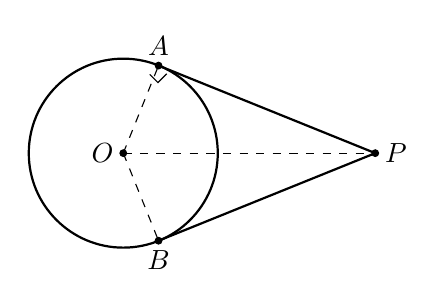
\begin{tikzpicture}[scale=0.8]
        \draw[thick] (0,0) circle (1.5cm);
        \coordinate (O) at (0,0);
        \coordinate (P) at (4,0);
        \coordinate (A) at (0.56, 1.39);
        \coordinate (B) at (0.56, -1.39);
        
        \draw[dashed] (O) -- (A);
        \draw[dashed] (O) -- (B);
        \draw[dashed] (O) -- (P);
        \draw[thick] (P) -- (A);
        \draw[thick] (P) -- (B);
        
        \filldraw (O) circle (1.5pt) node[left] {$O$};
        \filldraw (P) circle (1.5pt) node[right] {$P$};
        \filldraw (A) circle (1.5pt) node[above] {$A$};
        \filldraw (B) circle (1.5pt) node[below] {$B$};
        
        % Right angle symbol at A
        \draw (0.42,1.25) -- (0.55,1.12) -- (0.69,1.26);
    \end{tikzpicture}

\end{center}
Radius is perpendicular to the tangent at the point of contact:
\begin{align}
	\angle OAP = 90^\circ
	\iff \brak{\vec{O} - \vec{A}}^{\top}\brak{\vec{P} - \vec{A}} = 0
	\label{eq:EE26BTECH11225-tangent-perp}
\end{align}
Tangents drawn to a circle from an external point $P$ are equal in length:
\begin{align}
	PA = PB
	\label{eq:EE26BTECH11225-tangent-equal}
\end{align}
\solution
The tangent at $\vec{A}$ is the line $\vec{x} = \vec{A} + \lambda\vec{m}$. Its points of intersection with the circle $\norm{\vec{x} - \vec{O}}^2 = r^2$ satisfy
\begin{align}
	\norm{\vec{A} - \vec{O} + \lambda\vec{m}}^2 = r^2
	\implies \norm{\vec{m}}^2\lambda^2 + 2\lambda\,\vec{m}^{\top}\brak{\vec{A} - \vec{O}} = 0
\end{align}
using $\norm{\vec{A} - \vec{O}}^2 = r^2$. The roots are $\lambda = 0$ and $\lambda = -\frac{2\vec{m}^{\top}\brak{\vec{A} - \vec{O}}}{\norm{\vec{m}}^2}$. A tangent touches the circle at only one point, so both roots must be zero, yielding
$\vec{m}^{\top}\brak{\vec{A} - \vec{O}} = 0$, which is \eqref{eq:EE26BTECH11225-tangent-perp} since $\vec{P} - \vec{A}$ is along $\vec{m}$.
\\
Now,
\begin{align}
	\norm{\vec{P} - \vec{O}}^2
	&= \norm{\brak{\vec{P} - \vec{A}} + \brak{\vec{A} - \vec{O}}}^2
	\\
	&= \norm{\vec{P} - \vec{A}}^2 + 2\brak{\vec{P} - \vec{A}}^{\top}\brak{\vec{A} - \vec{O}} + r^2
	\\
	\implies PA^2 &= \norm{\vec{P} - \vec{O}}^2 - r^2
\end{align}
by \eqref{eq:EE26BTECH11225-tangent-perp}. The same steps give $PB^2 = \norm{\vec{P} - \vec{O}}^2 - r^2$, yielding \eqref{eq:EE26BTECH11225-tangent-equal}.

\item Pythagoras Theorem in a right-angled triangle $ABC$ with $\angle B = 90^\circ$:
\begin{align}
	\text{Hypotenuse}^2 = \text{Base}^2 + \text{Height}^2
	\iff
	\norm{\vec{A} - \vec{C}}^2 = \norm{\vec{A} - \vec{B}}^2 + \norm{\vec{C} - \vec{B}}^2
	\label{eq:EE26BTECH11225-pythagoras}
\end{align}
\solution
The right angle at $B$ means
\begin{align}
	\brak{\vec{A} - \vec{B}}^{\top}\brak{\vec{C} - \vec{B}} = 0
\end{align}
Writing $\vec{A} - \vec{C} = \brak{\vec{A} - \vec{B}} - \brak{\vec{C} - \vec{B}}$,
\begin{align}
	\norm{\vec{A} - \vec{C}}^2
	= \norm{\vec{A} - \vec{B}}^2 + \norm{\vec{C} - \vec{B}}^2 - 2\brak{\vec{A} - \vec{B}}^{\top}\brak{\vec{C} - \vec{B}}
\end{align}
yielding \eqref{eq:EE26BTECH11225-pythagoras}.

\item Fundamental trigonometric identities and standard ratios:
\begin{align}
	\sin^2 A + \cos^2 A &= 1
	\label{eq:EE26BTECH11225-trig-1}
	\\
	\sec^2 A - \tan^2 A &= 1
	\label{eq:EE26BTECH11225-trig-2}
	\\
	\csc^2 A - \cot^2 A &= 1
	\label{eq:EE26BTECH11225-trig-3}
\end{align}
For a vector $\vec{x} = \myvec{\text{Adjacent} \\ \text{Opposite}}$ making an angle $\theta$ with $\vec{e}_1$,
\begin{align}
	\begin{split}
		\sin\theta &= \frac{\text{Opposite}}{\text{Hypotenuse}} = \frac{\vec{e}_2^{\top}\vec{x}}{\norm{\vec{x}}}
		\\
		\cos\theta &= \frac{\text{Adjacent}}{\text{Hypotenuse}} = \frac{\vec{e}_1^{\top}\vec{x}}{\norm{\vec{x}}}
		\\
		\tan\theta &= \frac{\text{Opposite}}{\text{Adjacent}} = \frac{\vec{e}_2^{\top}\vec{x}}{\vec{e}_1^{\top}\vec{x}}
	\end{split}
	\label{eq:EE26BTECH11225-trig-ratios}
\end{align}
\solution
The point $\vec{r}\brak{A} = \myvec{\cos A \\ \sin A}$ lies on the unit circle, so
\begin{align}
	\norm{\vec{r}\brak{A}}^2 = \vec{r}\brak{A}^{\top}\vec{r}\brak{A} = \cos^2 A + \sin^2 A = 1
\end{align}
yielding \eqref{eq:EE26BTECH11225-trig-1}. Dividing by $\cos^2 A$ and $\sin^2 A$ respectively,
\begin{align}
	1 + \tan^2 A = \sec^2 A, \quad \cot^2 A + 1 = \csc^2 A
\end{align}
which are \eqref{eq:EE26BTECH11225-trig-2} and \eqref{eq:EE26BTECH11225-trig-3}.

\item Complementary angle identities:
\begin{align}
	\begin{split}
		\cos\brak{90^\circ - \theta} &= \sin\theta
		\\
		\tan\brak{90^\circ - \theta} &= \cot\theta
	\end{split}
	\label{eq:EE26BTECH11225-complementary}
\end{align}
\solution
Rotating the unit vector at angle $-\theta$ by $90^\circ$ using the rotation matrix,
\begin{align}
	\myvec{\cos\brak{90^\circ - \theta} \\ \sin\brak{90^\circ - \theta}}
	= \myvec{0 & -1 \\ 1 & 0}\myvec{\cos\theta \\ -\sin\theta}
	= \myvec{\sin\theta \\ \cos\theta}
\end{align}
yielding the first identity. Dividing the second row by the first,
\begin{align}
	\tan\brak{90^\circ - \theta} = \frac{\cos\theta}{\sin\theta} = \cot\theta
\end{align}

\item Area of a circular sector with central angle $\theta$:
\begin{align}
	\text{Area} = \frac{\theta}{360^\circ} \times \pi r^2
	\label{eq:EE26BTECH11225-sector}
\end{align}
\item Curved surface areas of a cylinder and a hemisphere of radius $r$:
\begin{align}
	\text{CSA of cylinder} &= 2\pi rh
	\label{eq:EE26BTECH11225-csa-cyl}
	\\
	\text{CSA of hemisphere} &= 2\pi r^2
	\label{eq:EE26BTECH11225-csa-hemi}
\end{align}
\item Volume, slant height, and curved surface area of a cone of base radius $r$ and height $h$:
\begin{align}
	V &= \frac{1}{3}\pi r^2 h
	\label{eq:EE26BTECH11225-cone-vol}
	\\
	l = \norm{\myvec{r \\ h}} &= \sqrt{r^2 + h^2}, \quad \text{CSA} = \pi r l
	\label{eq:EE26BTECH11225-cone-csa}
\end{align}
\solution
By similar triangles, the cross-section at height $z$ from the apex has radius $\frac{rz}{h}$. Integrating the areas of the circular cross-sections,
\begin{align}
	V = \int_{0}^{h}\pi\brak{\frac{rz}{h}}^2 dz = \frac{\pi r^2}{h^2}\sbrak{\frac{z^3}{3}}_{0}^{h} = \frac{1}{3}\pi r^2 h
\end{align}
The slant height is the length of the vector $\myvec{r \\ h}$. Cutting the cone along a slant line and unrolling it gives a sector of radius $l$ and arc length $2\pi r$, so the angle is $\theta_r = \frac{2\pi r}{l}$. From \eqref{eq:EE26BTECH11225-sector} in radians,
\begin{align}
	\text{CSA} = \frac{1}{2}l^2\theta_r = \pi r l
\end{align}

\item Slant height and surface area of an open frustum with radii $R > r$ and height $h$:
\begin{align}
	l = \norm{\myvec{R - r \\ h}} &= \sqrt{h^2 + \brak{R - r}^2}
	\label{eq:EE26BTECH11225-frustum-l}
	\\
	\text{Area} &= \pi\brak{R + r}l + \pi r^2
	\label{eq:EE26BTECH11225-frustum-area}
\end{align}
\solution
The slant height is the length of the vector $\myvec{R - r \\ h}$. Let $L$ be the slant height of the full cone of base radius $R$. The removed cone has radius $r$ and slant height $L - l$. By similar triangles,
\begin{align}
	\frac{r}{R} = \frac{L - l}{L}
	\implies L = \frac{lR}{R - r}
\end{align}
Subtracting the curved surface areas using \eqref{eq:EE26BTECH11225-cone-csa},
\begin{align}
	\text{CSA} = \pi RL - \pi r\brak{L - l}
	= \pi\sbrak{\brak{R - r}L + rl}
	= \pi\brak{R + r}l
\end{align}
Adding the circular base of radius $r$ yields \eqref{eq:EE26BTECH11225-frustum-area}.

\item Direct method for the mean and the grouped median formula, for class marks $x_i$ and frequencies $f_i$:
\begin{align}
	\bar{x} &= \frac{\sum f_i x_i}{\sum f_i} = \frac{\vec{f}^{\top}\vec{x}}{\vec{f}^{\top}\vec{1}}
	\label{eq:EE26BTECH11225-mean}
	\\
	\text{Median} &= l + \brak{\frac{\frac{N}{2} - cf}{f}} \times h
	\label{eq:EE26BTECH11225-median}
\end{align}
where $N = \sum f_i$, $l$ is the lower limit, $h$ the width and $f$ the frequency of the median class, and $cf$ the cumulative frequency of the class preceding it.
\\
\solution
The mean $m$ minimizes the weighted squared error
\begin{align}
	J\brak{m} = \sum f_i\brak{x_i - m}^2
	\implies \frac{dJ}{dm} = -2\sum f_i\brak{x_i - m} = 0
	\implies m = \frac{\sum f_i x_i}{\sum f_i}
\end{align}
yielding \eqref{eq:EE26BTECH11225-mean}. For the median, assuming the frequency is uniformly spread over the median class, the cumulative frequency is linear in that class,
\begin{align}
	F\brak{x} = cf + \frac{f}{h}\brak{x - l}
\end{align}
The median is the value where $F\brak{x} = \frac{N}{2}$,
\begin{align}
	\frac{N}{2} = cf + \frac{f}{h}\brak{x - l}
	\implies x = l + \brak{\frac{\frac{N}{2} - cf}{f}} \times h
\end{align}
yielding \eqref{eq:EE26BTECH11225-median}.

\item The unit step function, and an A.P. with first term $a$ and common difference $d$ written as a sequence:
\begin{align}
u(n) &= \begin{cases} 1, & n \ge 0 \\ 0, & n < 0 \end{cases} \label{eq:EE26BTECH11225-unit-step} \\
x(n) &= \brak{a + (n-1)d}\,u(n-1) \label{eq:EE26BTECH11225-ap-step}
\end{align}
Thus $x(n) = 0$ for $n < 1$ and $x(n) = a_n$ for $n \ge 1$.
\item Newton--Raphson iteration to find a root of $f(x) = 0$ from a starting value $x_0$:
\begin{align}
x_{n+1} = x_n - \frac{f(x_n)}{f'(x_n)}, \quad f'(x_n) \ne 0 \label{eq:EE26BTECH11225-newton}
\end{align}
\solution The tangent to $y = f(x)$ at $x = x_n$ is $y = f(x_n) + f'(x_n)(x - x_n)$. It meets the $x$-axis where $y = 0$, which gives $x_{n+1}$ above.
\item Probability mass function (PMF) of a discrete random variable $X$, and of a pair $(X,Y)$:
\begin{align}
p_X(k) &= \Pr\brak{X = k}, \quad \sum_k p_X(k) = 1, \quad \Pr\brak{X \in E} = \sum_{k \in E} p_X(k) \label{eq:EE26BTECH11225-pmf} \\
p_{XY}(i,j) &= p_X(i)\,p_Y(j) \quad \text{when $X$ and $Y$ are independent} \label{eq:EE26BTECH11225-pmf-joint}
\end{align}
\end{enumerate}
